\documentclass[12pt]{article}

\input{cs486_assign_preamble.tex}

\lhead{CS 486/686}
\chead{Fall 2022}
\rhead{Assignment 3}
\cfoot{v1.0}
\lfoot{\copyright Blake VanBerlo 2022}

\title{CS 486/686 Assignment 3 \\ Fall 2022 \\ (125 marks) }
\author{Blake VanBerlo}
\date{Due Date: 11:59 pm ET on Tuesday, November 15, 2022}

\begin{document}

\maketitle

% \section*{Changes}

% \begin{itemize}

% \end{itemize}

\newpage

\newpage
\section*{Instructions}

\begin{itemize}
\item
Submit the signed academic integrity statement any written solutions in a file to the Q0 box in the A3 project on Crowdmark. \textbf{(5 marks)}.

\item Submit your written answers to questions 1 and 2 as PDF files to the Q1 and Q2 boxes respectively in the A3 project on Crowdmark. I strongly encourage you to complete your write-up in LaTeX, using this source file. If you do, in your submission, please replace the author with your name and student number. Please also remove the due date, the Instructions section, and the Learning Goals section. Thank you!

\item Submit any code to \verb+Marmoset+ at \url{https://marmoset.student.cs.uwaterloo.ca/}. Be sure to submit your code to the project named \texttt{Assignment 3 - Final}. 

\item
No late assignment will be accepted. This assignment is to be done individually.

\item
Lead TAs: 
\begin{itemize}
\item 
Connor Raymond Stewart (\url{crstewart@uwaterloo.ca})
\item
Dake Zhang (\url{dake.zhang@uwaterloo.ca})
\end{itemize}
The TAs' office hours will be scheduled and posted on LEARN and Piazza.
\end{itemize}



\section*{Learning goals}

{\bf Hidden Markov Models (HHM)}
\begin{itemize}
    \item Derive the formula for the prediction inference task in HMMs
    \item Trace the forward-backward algorithm
\end{itemize}

{\bf Decision Trees}
\begin{itemize}
\item 
Implement the decision tree learner algorithm to learn a decision tree using a dataset with real-valued features.
\item
Determine the accuracy of a decision tree on a dataset.
\item
Perform pre-pruning and post-pruning. Determine the best parameter value for pruning using $k$-fold cross validation.
\end{itemize}




\newpage
\section{Hidden Markov Models (30 marks)}
\label{question_hmm}

\begin{enumerate}[font=\Large,label=(\alph*)]

\item
In Lectures 10 and 11, we used a different form of the Bayes rule in our derivations for the filtering and smoothing formulas. Show that $P(A\,|\,B \land C) = \alpha P(B\,|\,A \land C) P(A\,|\,C)$, where $\alpha$ is a normalizing constant. In your derivation, clearly identify any probability rules that you use (see the rules in Lecture 6).

\begin{markscheme}

(2 marks) Correct derivation

(2 marks) Correct rules cited

\end{markscheme}

\begin{sol}
    {\color{blue} 

        $P(A|B \land C) = P(A \land B \land C)/P(B \land C)$ - Bayes rule  

        $ = P(B| A \land C) P(A \land C) /P(B \land C)$ - Bayes rule  

        $ = P(B| A \land C) P(A|C) P(C) /P(B \land C)$ - Bayes rule  

        $ = \alpha P(B\,|\,A \land C) P(A\,|\,C)$ , where $\alpha  = P(C) /P(B \land C) $

    }   
    \end{sol}

\item
Several commodities have been experiencing volatile prices recently, often due to supply chain issues and product shortages. Olive oil is an example of a product that might experience product shortages this year due to \href{https://www.cnn.com/interactive/2022/09/business/olive-oil-shortage-drought-cnnphotos/}{droughts in Europe}.

Suppose that you would like to determine the state of olive oil availability, given the price that you observe during your weekly grocery shopping trip. You model this problem as a Hidden Markov Model (HMM), where the hidden state $S_t$ is the state of olive oil supply (normal, supply chain backup, or shortage) and the observation is the price you see in the grocery store for a \SI{1}{L} bottle (low, normal, high). You make some assumptions regarding the transition and sensor distributions. For 3 weeks, you take note of the olive oil price, obtaining the HMM shown below:

\begin{center}
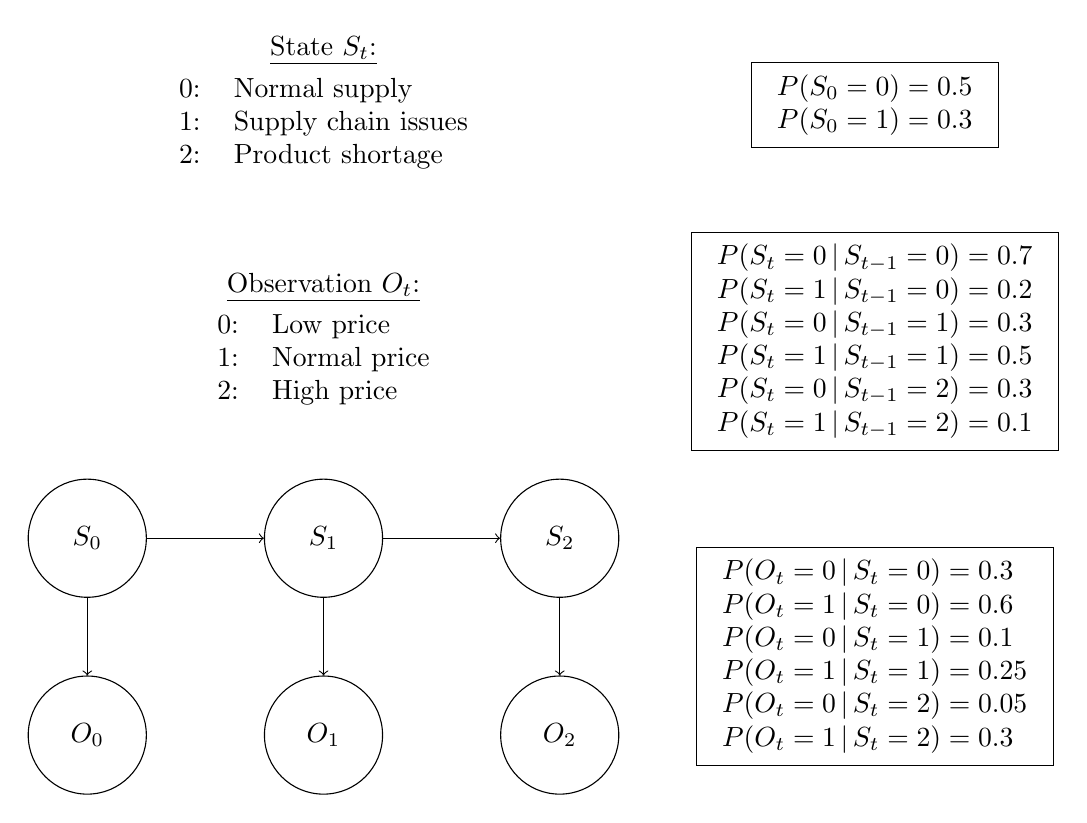
\begin{tikzpicture}[state/.style={circle, draw, minimum size=1.5cm}]

\node[draw] (tab1) at (10,10) {
\begin{tabular}{l}
$P(S_0=0) = 0.5$ \\
$P(S_0=1) = 0.3$ 
\end{tabular}
};

\node[draw] (tab2) at (10,7) {
\begin{tabular}{l}
$P(S_t=0 \,|\, S_{t-1}=0) = 0.7$ \\
$P(S_t=1 \,|\, S_{t-1}=0) = 0.2$ \\
$P(S_t=0 \,|\, S_{t-1}=1) = 0.3$ \\
$P(S_t=1 \,|\, S_{t-1}=1) = 0.5$ \\
$P(S_t=0 \,|\, S_{t-1}=2) = 0.3$ \\
$P(S_t=1 \,|\, S_{t-1}=2) = 0.1$ 
\end{tabular}
};

\node[draw] (tab3) at (10,3) {
\begin{tabular}{l}
$P(O_t=0 \,|\, S_t=0) =0.3$ \\
$P(O_t=1 \,|\, S_t=0) =0.6$ \\
$P(O_t=0 \,|\, S_t=1) =0.1$ \\
$P(O_t=1 \,|\, S_t=1) =0.25$ \\
$P(O_t=0 \,|\, S_t=2) =0.05$ \\
$P(O_t=1 \,|\, S_t=2) =0.3$ 
\end{tabular}
};

\node (rvs) at (3,10) {
\shortstack{ \underline{State $S_t$:} \\
\begin{tabular}{ll}
$0$: & Normal supply \\
$1$: & Supply chain issues \\
$2$: & Product shortage \\
\end{tabular}}
};

\node (rvs) at (3,7) {
\shortstack{ \underline{Observation $O_t$:} \\
\begin{tabular}{ll}
$0$: & Low price \\
$1$: & Normal price \\
$2$: & High price \\
\end{tabular}}
};

\node[state] (a) at (0, 4.5) {$S_0$};
\node[state] (b) at (3, 4.5) {$S_1$};
\node[state] (c) at (6, 4.5) {$S_2$};
\path[draw] [->] (a) -- (b);
\path[draw] [->] (b) -- (c);

\node[state] (e) at (0, 2) {$O_0$};
\node[state] (f) at (3, 2) {$O_1$};
\node[state] (g) at (6, 2) {$O_2$};
\path[draw] [->] (a) -- (e);
\path[draw] [->] (b) -- (f);
\path[draw] [->] (c) -- (g);

\end{tikzpicture}
\end{center}

You observed that the price of olive oil was normal in week $0$, high in week $1$, and high in week $2$. Execute the Forward Backward Algorithm to determine the probability distribution for the hidden state at each of weeks $0$, $1$, and $2$. That is, calculate $P(S_0 \,|\, O_0=1 \land O_1=2 \land O_2=2)$, $P(S_1 \,|\, O_0=1 \land O_1=2 \land O_2=2)$, and \\ $P(S_2 \,|\, O_0=1 \land O_1=2 \land O_2=2)$. Normalize each forward message. Show all calculations and round each calculation to $4$ decimal places. 

\begin{markscheme}

(10 marks) Correct execution of the Forward Backward Algorithm

(2 marks) \, Calculations are displayed clearly

\end{markscheme}

\begin{sol}
    {\color{blue} 

        Refer to attached image

    }   
    \end{sol}

\item 
Recall that \textit{prediction} in Hidden Markov Models is the task of computing the probability distribution for the hidden state at some future time step. More specifically, prediction computes the distribution $P(S_k\,|\,o_{0:t})$, where $t$ is the current time step and $k$ is some future time step ($k > t$). 

Given the state distribution for time step $k \geq t$, show that the distribution for the state at time step $k + 1$ can be recursively computed as follows:

\begin{align*}
    P(S_{k+1}\,|\,o_{0:t}) = \sum_{s_k} P(S_{k+1}\,|\,s_k) P(s_k\,|\,o_{0:t})
\end{align*}

In your derivation, clearly identify any conditional independence assumptions and/or probability rules that you use.

\begin{markscheme}

(6 marks) Correct derivation

(2 marks) Correct rules/assumptions cited

\end{markscheme}

\begin{sol}
    {\color{blue} 

        empty

    }   
    \end{sol}

\item
After many time steps (i.e., the \textit{mixing time}), the distribution returned by prediction will converge to a fixed point. In other words, once convergence is reached, $P(S_{k}\,|\,o_{0:t})$ does not change as $k$ increases. This distribution is referred to as the \textit{stationary distribution} of the HMM.

What is the stationary distribution of the HMM in Question 1(b)? Show your calculations.

\begin{markscheme}

(4 marks) Correct answer and justification

(2 marks) Calculations are displayed clearly

\end{markscheme}

\begin{sol}
    {\color{blue} 

        empty

    }   
    \end{sol}
    
\end{enumerate}

\end{document}





























